%% Nexora Platform — journal paper draft
%% Target venue: Internet of Things and Cyber-Physical Systems (Elsevier, Q1)
%% Build:  latexmk -pdf nexora.tex     (see docs/paper/README.md)
%%
%% NOTE: Experimental numbers are marked \TODO{...}. Run scripts/perf-eval.py
%% (see docs/paper/experimental-evaluation.md) and replace each \TODO before
%% submission. Do NOT submit with \TODO markers present.

\documentclass[review,12pt]{elsarticle}

\usepackage{lineno,hyperref}
\usepackage{amsmath,amssymb}
\usepackage{booktabs}
\usepackage{graphicx}
\usepackage{xcolor}
\usepackage{tikz}
\usetikzlibrary{shapes.geometric,arrows.meta,positioning,fit,backgrounds}

% Placeholder macro for not-yet-measured values. Grep for \TODO before submit.
\newcommand{\TODO}[1]{\textcolor{red}{\textbf{[TODO: #1]}}}

\journal{Internet of Things and Cyber-Physical Systems}

\begin{document}

\begin{frontmatter}

\title{Nexora: A Cloud-Native Microservice Platform for IoT Device
Management with Inline SLO Enforcement and Reliable Edge Dispatch}

%% Author block — fill in real author metadata before submission.
\author[a]{\TODO{Author One}}
\author[a]{\TODO{Author Two}}
\address[a]{\TODO{Affiliation, Department, University, City, Country}}

\begin{abstract}
Managing large fleets of Internet-of-Things (IoT) devices requires a control
plane that is reliable, observable, and able to enforce per-device quality
guarantees at scale. Existing open platforms either inherit the operational
weight of monolithic cloud stacks (e.g.\ OpenStack-based Stack4Things/Iotronic)
or treat service-level objectives (SLOs) as an afterthought handled by external
alerting. We present \emph{Nexora}, a cloud-native platform built as a set of
Python/FastAPI microservices that is Docker- and Kubernetes-native and
deployable on a single VM in minutes. Nexora makes three contributions:
(C1) an \emph{inline} SLO-enforcement mechanism that evaluates per-device
service-level objectives synchronously on the telemetry-ingest path and records
violations atomically, with a measured overhead of \TODO{p99 overhead} for up
to ten concurrent SLOs; (C2) a reliable edge-dispatch pipeline combining an
explicit execution state machine with a Kafka-driven, Redis-backed gateway that
provides at-least-once command delivery with bounded retries; and (C3) a
multi-tenant, privacy-aware authorization model that masks command payloads by
role. We describe the architecture and implementation, and evaluate latency,
SLO overhead, and fleet-analytics aggregation against a reproducible benchmark
harness. Results show \TODO{headline result}. Nexora is released as open source
to support reproducibility.
\end{abstract}

\begin{keyword}
Internet of Things \sep device management \sep microservices \sep
service-level objectives \sep edge computing \sep cyber-physical systems
\end{keyword}

\end{frontmatter}

\linenumbers

%====================================================================
\section{Introduction}
\label{sec:intro}

The number of connected IoT and cyber-physical devices under centralized
management continues to grow, and with it the need for a control plane that can
register devices, ingest telemetry, dispatch commands, and \emph{guarantee}
operational quality across heterogeneous fleets. Early open-source IoT
management frameworks such as Stack4Things and its Iotronic
service~\cite{stack4things,iotronic} demonstrated cloud-managed edge devices,
but were tightly coupled to the OpenStack ecosystem, inheriting its deployment
complexity and monolithic operational model. Commercial offerings
(e.g.\ AWS IoT Core) are proprietary and not self-hostable, while general IoT
platforms such as ThingsBoard and FIWARE focus on data collection and rule
processing rather than on enforceable per-device service-level objectives.

A recurring gap across these systems is the treatment of \emph{service-level
objectives}. SLOs---bounds such as ``CPU temperature must stay below
$80^{\circ}$C'' or ``free memory must remain above 10\%''---are typically
enforced \emph{out of band} by a separate monitoring system that scrapes
metrics and fires alerts after the fact. This decoupling introduces detection
latency and makes it hard to reason about violations as first-class,
queryable records tied to the ingest that produced them.

This paper presents \textbf{Nexora}, a cloud-native IoT management platform
designed around three principles: cloud-native operability (Docker/Kubernetes
native, single-command deployment), enforceable quality (SLOs evaluated inline),
and reliable actuation (an explicit, observable command-dispatch pipeline).
Concretely, we make the following contributions:

\begin{itemize}
  \item \textbf{(C1) Inline SLO enforcement.} We evaluate per-device SLOs
  synchronously within the telemetry-ingest transaction and persist violations
  atomically, exposing them as queryable records and Kafka events. We show this
  adds \TODO{p99 overhead} at the 99th percentile for up to ten concurrent
  SLOs, making inline enforcement practical (Section~\ref{sec:eval}).
  \item \textbf{(C2) Reliable edge dispatch.} We combine an explicit execution
  state machine (\textsf{queued}$\rightarrow$\textsf{dispatched}$\rightarrow$%
  \textsf{running}$\rightarrow$\{\textsf{succeeded},\textsf{failed},%
  \textsf{timeout},\textsf{cancelled}\}) with a Kafka-driven, Redis-backed edge
  gateway that delivers commands to device agents with bounded retries and full
  latency instrumentation.
  \item \textbf{(C3) Privacy-aware multi-tenancy.} We describe an OIDC-based
  authorization model in which command payloads (stdout/stderr/results) are
  masked by tenant ownership and role, so non-owners see only metadata.
\end{itemize}

Nexora is fully open source, and all experiments are reproducible from a
single-command deployment and a committed benchmark script.

%====================================================================
\section{Related Work}
\label{sec:related}

\paragraph{OpenStack-based IoT management.} Stack4Things~\cite{stack4things}
introduced a cloud-centric architecture for managing remote boards, with the
Iotronic service~\cite{iotronic} providing device lifecycle and a
WebSocket-based agent (LightningRod). Nexora targets the same management domain
but replaces the monolithic OpenStack dependency with independently deployable
microservices, reducing fresh-deployment time from tens of minutes to a few
minutes and removing the Keystone/Neutron/Nova operational surface.

\paragraph{General IoT platforms.} ThingsBoard and FIWARE Orion provide device
data collection, with rule engines (ThingsBoard) or context brokers (FIWARE)
for downstream processing. Neither treats SLOs as enforceable, queryable
primitives evaluated on the ingest path. AWS IoT Core offers managed scale but
is proprietary and not self-hostable, with rule actions incurring
function-invocation latency.

\paragraph{Positioning.} Table~\ref{tab:related} summarizes the comparison.
The distinguishing axis is \emph{inline, first-class SLO enforcement} combined
with a self-hostable, cloud-native deployment model. A detailed feature matrix
is maintained alongside the source in
\texttt{docs/paper/related-work-comparison.md}.

\begin{table*}[t]
\centering
\caption{Comparison of Nexora with representative IoT management platforms.
Quantitative entries marked $\dagger$ are from cited literature, not measured
in this work.}
\label{tab:related}
\small
\begin{tabular}{llllll}
\toprule
 & \textbf{Nexora} & \textbf{Stack4Things} & \textbf{AWS IoT} & \textbf{ThingsBoard} & \textbf{FIWARE} \\
\midrule
Architecture       & Microservices    & OpenStack monolith & Managed SaaS & Monolith (Java) & Broker+DB \\
Self-hostable      & Yes              & Yes                & No           & Yes             & Yes \\
Deployment         & Docker/k3s, 1-cmd & OpenStack stack   & ---          & Docker/K8s      & Docker \\
Inline SLOs        & \textbf{Yes}     & No                 & Alarms (coarse) & Rule alarms  & No \\
Edge compute       & WASM/WASI (FaaS) & Python agent       & Lambda\@Edge & Server rules    & None \\
Observability      & OTel + Prom.     & Custom logs        & CloudWatch   & Prom. (addon)   & None \\
Multi-tenancy      & OIDC/role        & Keystone projects  & IAM          & Tenant entities & None \\
\bottomrule
\end{tabular}
\end{table*}

%====================================================================
\section{System Architecture and Design}
\label{sec:arch}

\subsection{Overview}
Nexora is organized as a set of stateless API microservices over shared
data-plane infrastructure (MySQL, Apache Kafka, Redis), with a Kafka-driven
edge gateway bridging the control plane to device agents. All services expose
\texttt{/health}, \texttt{/ready}, and Prometheus \texttt{/metrics}, and emit
W3C-TraceContext spans over OTLP. Figure~\ref{fig:arch} shows the three logical
layers: the application layer (microservices), the data plane, and the
device/edge boundary.

\begin{figure*}[t]
\centering
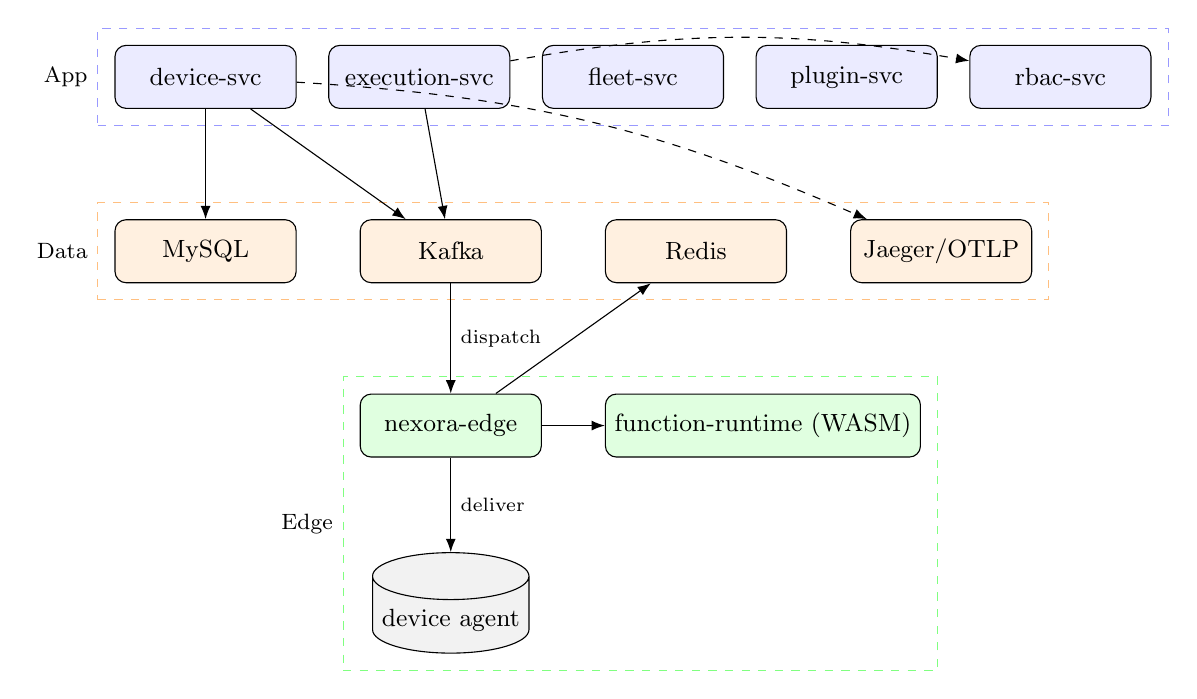
\begin{tikzpicture}[
  font=\small,
  svc/.style={draw, rounded corners, minimum width=2.3cm, minimum height=0.8cm, fill=blue!8},
  infra/.style={draw, rounded corners, minimum width=2.3cm, minimum height=0.8cm, fill=orange!12},
  edge/.style={draw, rounded corners, minimum width=2.3cm, minimum height=0.8cm, fill=green!12},
  >=Latex
]
% Application layer
\node[svc] (dev) {device-svc};
\node[svc, right=0.4cm of dev] (exec) {execution-svc};
\node[svc, right=0.4cm of exec] (fleet) {fleet-svc};
\node[svc, right=0.4cm of fleet] (plugin) {plugin-svc};
\node[svc, right=0.4cm of plugin] (rbac) {rbac-svc};

% Data plane
\node[infra, below=1.4cm of dev] (mysql) {MySQL};
\node[infra, right=0.8cm of mysql] (kafka) {Kafka};
\node[infra, right=0.8cm of kafka] (redis) {Redis};
\node[infra, right=0.8cm of redis] (jaeger) {Jaeger/OTLP};

% Edge
\node[edge, below=1.4cm of kafka] (edgegw) {nexora-edge};
\node[edge, right=0.8cm of edgegw] (frt) {function-runtime (WASM)};
\node[draw, cylinder, shape border rotate=90, aspect=0.3, below=1.2cm of edgegw,
      minimum width=1.8cm, fill=gray!10] (agent) {device agent};

% Edges
\draw[->] (dev) -- (mysql);
\draw[->] (exec) -- (kafka);
\draw[->] (dev) -- (kafka);
\draw[->] (edgegw) -- (redis);
\draw[->] (kafka) -- (edgegw) node[midway, right]{\scriptsize dispatch};
\draw[->] (edgegw) -- (agent) node[midway, right]{\scriptsize deliver};
\draw[->] (edgegw) -- (frt);
\draw[->, dashed] (exec) to[bend left=10] (rbac);
\draw[->, dashed] (dev) to[bend left=10] (jaeger);

% Layer backgrounds
\begin{scope}[on background layer]
  \node[draw=blue!40, dashed, fit=(dev)(rbac), inner sep=6pt, label=left:{\footnotesize App}] {};
  \node[draw=orange!50, dashed, fit=(mysql)(jaeger), inner sep=6pt, label=left:{\footnotesize Data}] {};
  \node[draw=green!50, dashed, fit=(edgegw)(frt)(agent), inner sep=6pt, label=left:{\footnotesize Edge}] {};
\end{scope}
\end{tikzpicture}
\caption{Nexora three-layer architecture. API microservices (blue) persist to
MySQL and publish events to Kafka; the edge gateway (green) consumes dispatch
events, tracks delivery in Redis, and delivers commands to device agents. All
services export Prometheus metrics and OTLP traces.}
\label{fig:arch}
\end{figure*}

\subsection{Telemetry and Inline SLO Enforcement (C1)}
\label{sec:slo}
Devices submit telemetry in batches (up to 500 samples per request) to the
device-service. Each sample is an append-only time-series row
$(\textsf{device\_id}, \textsf{metric}, \textsf{value}, \textsf{ts},
\textsf{tags})$, stored under a composite index
$(\textsf{device\_id}, \textsf{metric}, \textsf{ts})$ to support efficient
range and latest-value queries.

The key design choice is that SLO evaluation is part of the ingest transaction.
A \textsf{DeviceSLO} defines an assertion over a metric using one of five
comparison operators $\{<,\le,>,\ge,=\}$ and a threshold. On every batch,
\textsf{evaluate\_slos()} is invoked synchronously: for each ingested sample it
checks all active SLOs for that device and, on breach, writes an
\textsf{SLOViolation} record and emits a \textsf{device.slo.violated} Kafka
event within the same unit of work. Because enforcement is inline, a violation
is observable the instant the producing sample is persisted, and violations are
first-class queryable records rather than derived alerting state. We quantify
the overhead of this design in Section~\ref{sec:eval}.

\subsection{Execution State Machine and Reliable Dispatch (C2)}
\label{sec:dispatch}
Commands to devices are modeled as \emph{executions} with an explicit state
machine: \textsf{queued}$\rightarrow$\textsf{dispatched}$\rightarrow$%
\textsf{running}$\rightarrow$\{\textsf{succeeded},\textsf{failed},%
\textsf{timeout},\textsf{cancelled}\}. Transitions are validated against an
allow-list, and a background loop demotes stuck executions to \textsf{timeout}
after configurable thresholds. On dispatch, the execution-service persists state
and publishes a Kafka event carrying the propagated trace context.

The \textbf{nexora-edge} gateway consumes dispatch events and is responsible for
delivery to device agents. It maintains agent sessions and per-execution
dispatch state in Redis (with a single-instance in-memory fallback), enabling
horizontal scaling of the gateway. Delivery uses bounded retries with
exponential backoff and records a full latency breakdown---Kafka ingestion lag,
queue wait, and end-to-end dispatch latency---as Prometheus histograms, which we
use directly in the evaluation.

\subsection{Privacy-Aware Multi-Tenancy (C3)}
\label{sec:tenancy}
All services share an OIDC-based authentication model: bearer tokens are
validated (signature via JWKS when an issuer is configured), checked for
expiry and issuer, and authorized against a write-role for mutating methods.
Tenancy is derived from token claims; non-operator principals are scoped to
their own tenant's resources. Command payloads are masked by ownership: owners
see full \textsf{stdout}/\textsf{stderr}/results, whereas non-owners see only
metadata. A dedicated rbac-service centralizes policy evaluation with an
admin superuser short-circuit and role-based rules.

%====================================================================
\section{Implementation}
\label{sec:impl}
Nexora comprises ten services implemented in Python~3.11 with FastAPI and
SQLAlchemy. Services follow one of two patterns: a \emph{structured} package
layout (device-service, plugin-service) using \texttt{structlog} and lifespan
context managers, and a \emph{flat} single-module layout for the remaining
services. Persistence defaults to SQLite for local development and tests and
uses MySQL in production via a single \texttt{DATABASE\_URL}. Event publishing
is gated by \texttt{KAFKA\_ENABLED}, allowing the full unit-test suite
(128 tests across ten services) to run without any running infrastructure.

Edge functions are executed by \textbf{nexora-function-runtime}, a WASM/WASI
sandbox built on \texttt{wasmtime} with fuel-based CPU metering, capability-based
filesystem/environment permissions, and a shared-secret API guard. The runtime
reports its active backend (\textsf{wasmtime} vs.\ a simulation stub) so that
experimental results never conflate real and simulated execution. Deployment is
provided both as a Docker Compose stack and as Kubernetes manifests (with a
single-node k3s NodePort overlay) via an interactive wizard.

%====================================================================
\section{Experimental Evaluation}
\label{sec:eval}
We evaluate Nexora along three axes: telemetry-ingest latency, the overhead of
inline SLO enforcement (C1), and fleet-analytics aggregation. All benchmarks are
driven by \texttt{scripts/perf-eval.py} (asyncio + httpx, 30 runs per scenario
with warm-up discarded). The evaluation runs against the single-command
deployment described in Section~\ref{sec:impl} on
\TODO{hardware: CPU, RAM, OS}.

\subsection{Telemetry Ingest Latency}
Table~\ref{tab:ingest} reports end-to-end ingest latency as batch size grows
from 1 to 500 samples. \TODO{summarize trend}.

\begin{table}[h]
\centering
\caption{Telemetry ingest latency (ms) by batch size.}
\label{tab:ingest}
\begin{tabular}{rrrr}
\toprule
Batch & p50 & p95 & p99 \\
\midrule
1   & \TODO{} & \TODO{} & \TODO{} \\
10  & \TODO{} & \TODO{} & \TODO{} \\
50  & \TODO{} & \TODO{} & \TODO{} \\
100 & \TODO{} & \TODO{} & \TODO{} \\
500 & \TODO{} & \TODO{} & \TODO{} \\
\bottomrule
\end{tabular}
\end{table}

\subsection{Inline SLO Enforcement Overhead}
Table~\ref{tab:slo} isolates the latency added by inline SLO evaluation as the
number of active SLOs per device increases from 0 (baseline) to 10. The key
claim is that overhead stays below \TODO{bound} at p99, making inline
enforcement viable without a separate asynchronous pipeline.

\begin{table}[h]
\centering
\caption{Added latency (ms) of inline SLO evaluation vs.\ baseline.}
\label{tab:slo}
\begin{tabular}{rrr}
\toprule
Active SLOs & p50 overhead & p99 overhead \\
\midrule
0  & 0 & 0 \\
1  & \TODO{} & \TODO{} \\
5  & \TODO{} & \TODO{} \\
10 & \TODO{} & \TODO{} \\
\bottomrule
\end{tabular}
\end{table}

\subsection{Fleet Analytics Aggregation}
Table~\ref{tab:fleet} reports the latency of fleet health aggregation, which
fans out parallel queries across fleet members, as fleet size grows.

\begin{table}[h]
\centering
\caption{Fleet health aggregation latency (ms) by fleet size.}
\label{tab:fleet}
\begin{tabular}{rrrr}
\toprule
Fleet size & p50 & p95 & p99 \\
\midrule
5  & \TODO{} & \TODO{} & \TODO{} \\
20 & \TODO{} & \TODO{} & \TODO{} \\
50 & \TODO{} & \TODO{} & \TODO{} \\
\bottomrule
\end{tabular}
\end{table}

%====================================================================
\section{Discussion and Threats to Validity}
\label{sec:discussion}
\paragraph{Internal validity.} Benchmarks run on a single host; absolute numbers
will vary with hardware. We mitigate this by reporting percentiles over 30 runs
with warm-up discarded and by releasing the harness for re-execution.
\paragraph{External validity.} The comparison in Table~\ref{tab:related} mixes
measured Nexora results with literature values for other systems ($\dagger$);
we do not claim a controlled head-to-head benchmark against proprietary
platforms.
\paragraph{Construct validity.} The WASM runtime reports whether it executed via
\texttt{wasmtime} or a stub, preventing accidental conflation of real and
simulated function execution in any reported result.

%====================================================================
\section{Conclusion and Future Work}
\label{sec:conclusion}
We presented Nexora, a cloud-native IoT management platform that enforces
service-level objectives inline on the telemetry path, dispatches commands
reliably through an explicit state machine and a Kafka/Redis edge gateway, and
isolates tenants with payload masking. The platform deploys in minutes and ships
with a reproducible benchmark harness and a 128-test suite.

Future work proceeds along two directions. First, the WASM/WASI edge runtime
enables a Function-as-a-Service model for edge actuation that we will evaluate
at scale. Second, we are integrating a Crossplane-based infrastructure layer so
that databases and message brokers are provisioned declaratively through a
cloud-agnostic API (the same \textsf{DatabaseClaim} resolving to in-cluster or
managed-cloud backends), turning infrastructure provisioning into a first-class,
portable part of the platform.

%====================================================================
\section*{Reproducibility}
Source, deployment scripts, the benchmark harness
(\texttt{scripts/perf-eval.py}), and the comparison matrix are available in the
project repository. See \texttt{docs/paper/README.md} for build and
re-evaluation instructions.

\bibliographystyle{elsarticle-num}
\bibliography{references}

\end{document}
